\documentclass[12pt]{article}
\usepackage[utf8]{inputenc}
\usepackage{minted}
\usepackage{multirow}
\usepackage{listings}
\usepackage{amssymb,amsmath,amsthm,amsfonts}
\usepackage{graphicx}
\usepackage{titlesec}
\usepackage{gensymb}
\usepackage{url}
\usepackage{fancyhdr}
\usepackage[spanish]{babel}
\usepackage[nolist]{acronym}
\usepackage[table]{xcolor}
\usepackage{url}
\usepackage{float}

% HYPERLINK CONFIGURATION %
\usepackage[colorlinks=true, allcolors=blue]{hyperref}
\hypersetup{
    colorlinks=true,% make the links colored
}
    
% MARGINS CONFIGURATION %
\usepackage{vmargin}
\setmarginsrb{2 cm}{2 cm}{2 cm}{2 cm}{1 cm}{1.5 cm}{1 cm}{1.5 cm}

% GRAPHICS CONFIGURATION %
\usepackage{graphicx}
\graphicspath{{images/}}

\begin{document}

\begin{titlepage}

    \title{     \textbf{Propuesta de Tesis de Grado \\ de Ingeniería en Informática}\\[2.5ex]
        \textit{Detección de Deadlocks en Rust \\en tiempo de compilación \\mediante Redes de Petri} }

    \author{
        \textbf{Director:} Ing. Pablo A. Deymonnaz\\[2.5ex]
        \textbf{Alumno:} Horacio Lisdero Scaffino, \textit{(Padrón \# 100.132)}                                \\
        \texttt{ hlisdero@fi.uba.ar }                                    \\[2.5ex]
        \normalsize{Facultad de Ingeniería, Universidad de Buenos Aires}        \\
    }

    \date{17 de febrero de 2023}

\end{titlepage}

\maketitle
\thispagestyle{empty}

\maketitle{
    \hypersetup{linkcolor=black}
    \tableofcontents
}

\section{Introducción}

\subsection{El problema de la correctitud en programación concurrente}

En el área de computación concurrente, uno de los desafíos principales es probar la correctitud de un programa concurrente.
A diferencia de un programa secuencial donde para cada entrada se obtiene siempre la misma salida, en un programa concurrente
la salida puede depender de cómo se intercalaron las instrucciones de los diferentes procesos o threads durante la ejecución.

La correctitud de un programa concurrente se define entonces en términos de propiedades del cómputo realizado y no en términos del
resultado obtenido. En la literatura \cite{ben-ari2006, coulouris2012, tanenbaum2017} se definen dos tipos de propiedades de correctitud:

\begin{itemize}
    \item Propiedades de \textit{safety}: Propiedades que se deben cumplir \textit{siempre}.
    \item Propiedades de \textit{liveness}: Propiedades que se deben cumplir \textit{eventualmente}.
\end{itemize}

Dos de las propiedades de tipo \textit{safety} deseables en un programa concurrente son:

\begin{itemize}
    \item \textbf{Exclusión mutua}: dos procesos no deben acceder a recursos compartidos al mismo tiempo.
    \item \textbf{Ausencia de \textit{deadlock}}: un sistema en ejecución debe poder continuar realizando su tarea, es decir, avanzar produciendo trabajo útil.
\end{itemize}

Usualmente se utilizan primitivas de sincronización tales como mutexes, semáforos, monitores y \textit{condition variables}
para implementar el acceso coordinado de los procesos o hilos a los recursos compartidos.
No obstante, el uso correcto de estas primitivas es difícil de lograr en la práctica y se pueden introducir errores difíciles de detectar y corregir.
Actualmente la mayoría de lenguajes de uso general, ya sean compilados o interpretados, no permiten detectar estos errores en todos los casos.

Dada la creciente importancia de la programación concurrente debida a la proliferación de sistemas de hardware multihilo y multiproceso,
reducir el número de \textit{bugs} ligados a la sincronización de los procesos o hilos es de vital importancia para la industria.
Evitar los \textit{deadlocks} es un requerimiento ineludible en el desarrollo, especialmente en sistemas embebidos y sistemas de misión crítica como vehículos autónomos o aeronaves.

\subsection{Redes de Petri}

Las redes de Petri son una herramienta gráfica y matemática ampliamente utilizada para describir sistemas distribuidos \cite{murata1989}.
Fueron introducidas por el investigador alemán Carl Adam Petri en su tesis de doctorado en 1962 \cite{petri1962}.
Una red de Petri consiste en un grafo dirigido bipartito, el cual cuenta con dos tipos de nodos: lugares (\textit{places}) y transiciones (\textit{transitions}).
Únicamente pueden existir arcos dirigidos entre un lugar y una transición o entre una transición y un lugar.
A los lugares se les asignan marcas (\textit{tokens}) los cuales representan el estado actual del sistema o un recurso en particular.

\begin{figure}[H]
    \centering
    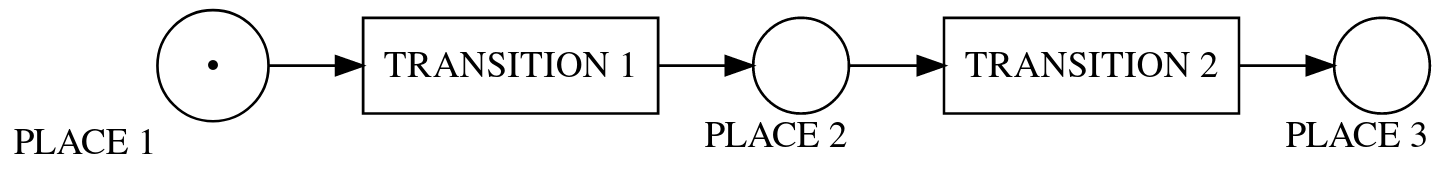
\includegraphics[scale=0.25]{petri-net-example.png}
    \caption{Ejemplo de una red de Petri. \texttt{PLACE 1} contiene un \textit{token}.}
\end{figure}

Las transiciones se disparan siguiendo la siguiente regla:
\begin{itemize}
    \item Se consume un \textit{token} de los lugares cuyos arcos entran a la transición.
    \item Se crea un token en cada lugar al cual llega un arco saliente de la transición.
\end{itemize}

\begin{figure}[H]
    \centering
    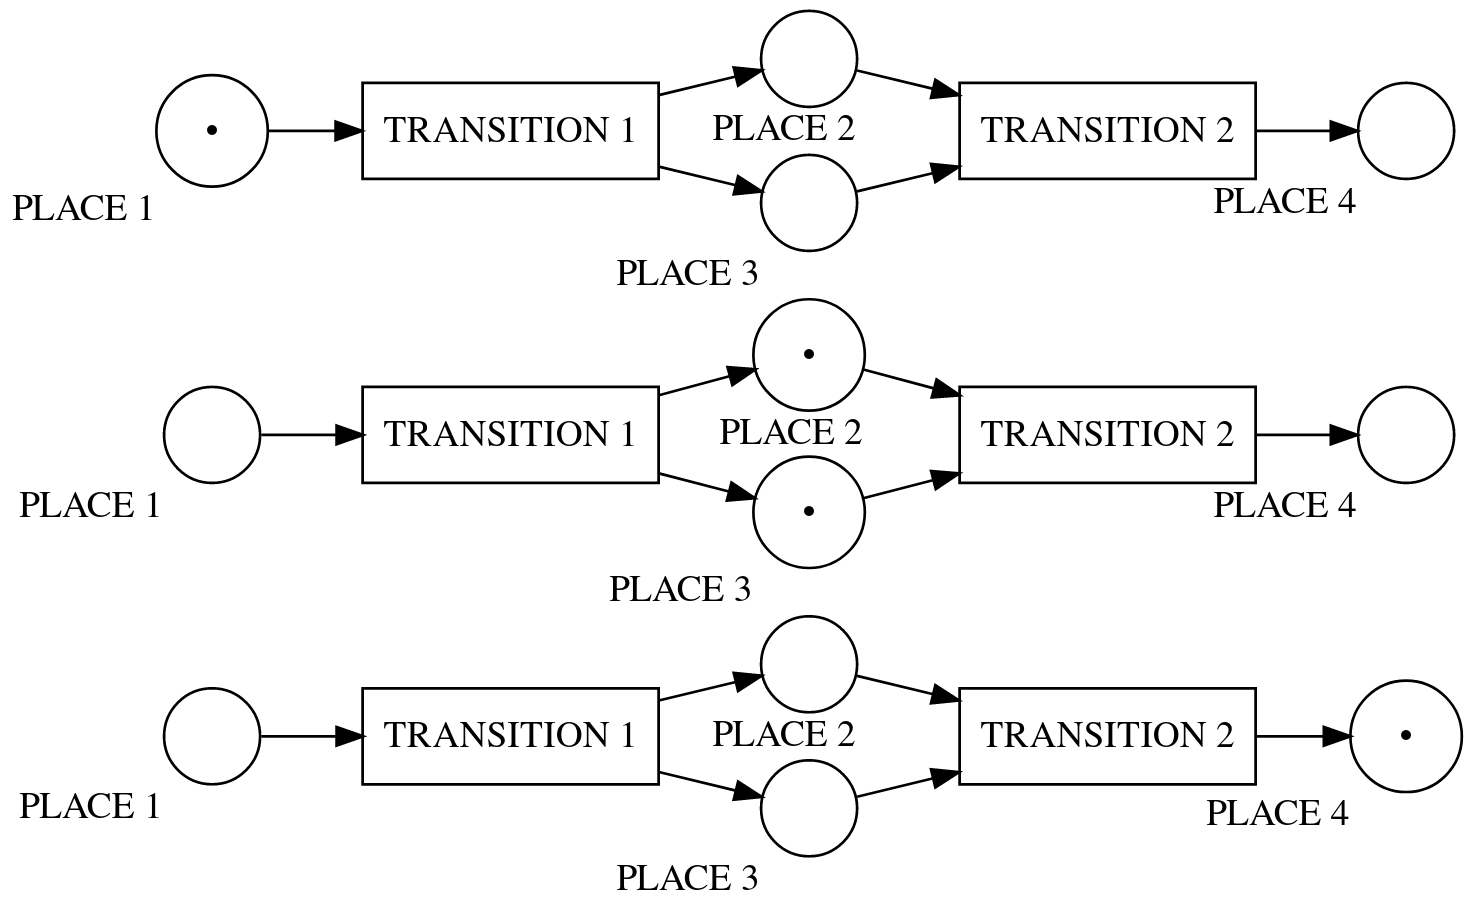
\includegraphics[scale=0.25]{petri-net-transition-firing-example.png}
    \caption{Ejemplo de disparo de transiciones. Primero se dispara la transición 1 y luego la transición 2.}
\end{figure}

Las redes de Petri pueden ser vistas como una versión generalizada de las máquinas de estado que permite modelar la concurrencia y el paralelismo.

\subsection{Motivación}

En el presente trabajo nos proponemos estudiar la detección de \textit{deadlocks} y \textit{lost signals} en el lenguaje de programación Rust.
Se utilizará un modelo teórico basado en Redes de Petri para encontrar los errores en el código fuente. Mediante una traducción del código fuente
en tiempo de compilación, se obtendrá una red de Petri que luego podrá ser analizada mediante métodos de verificación de modelos para garantizar la ausencia de \textit{deadlocks}.

El trabajo contará con una primera implementación del traductor que podrá ser utilizado como \textit{plugin} del gestor de paquetes estándar de Rust \textit{cargo} \cite{cargo-website}.
El objetivo es contribuir a la comunidad de Rust aportando una primera versión de esta herramienta que podría luego ser extendida para soportar casos más complejos.
Se busca que el uso de la herramienta sea lo más sencillo y accesible posible para fomentar su uso y aplicación a proyectos reales de software.
A largo plazo, se podría incorporar la herramienta al compilador como un pase adicional opcional en el proceso de compilación.
Este pase verificaría que no se pueden producir deadlocks, lo que haría de Rust un lenguaje de programación aún más seguro y confiable.

\bigskip

\section{Estado del arte / Literatura relacionada}

\subsection{El lenguaje de programación Rust}

Uno de los lenguajes de programación modernos más prometedores para programación concurrente es Rust \cite{rust-website}.
Su modelo de memoria basado en el concepto de \textit{ownership} y su expresivo sistema de tipos permite eliminar una amplia variedad de
errores relacionados al manejo de memoria y a la programación concurrente en tiempo de compilación:

\begin{itemize}
    \item \textit{double free} \cite{rust-book-ownership}
    \item \textit{use-after-free} \cite{rust-book-ownership}
    \item referencia colgante "\textit{dangling pointers}" \cite{rust-book-references}
    \item \textit{data races} \cite{rust-book-references}
    \item pasaje de variables de tipo \textit{non-thread-safe} entre hilos \cite{rust-book-extensible-concurrency}
\end{itemize}

La importancia de estas ventajas para la industria no puede ser subestimada.
Diversas investigaciones empíricas han llegado a la conclusión que 70\% de las vulnerabilidades
encontradas en proyectos grandes en C/C++ ocurren debido a errores en el manejo de la memoria.
Esta cifra elevada se puede observar en proyectos tales como Android \cite{memory-bugs-android},
los componentes de Bluetooth y media de Android \cite{memory-bugs-android-media-bluetooth},
Chrome \cite{memory-bugs-chrome}, el componente CSS de Firefox \cite{memory-bugs-firefox},
iOS y macOS \cite{memory-bugs-ios-macos}, productos de Microsoft \cite{miller-security-microsoft2019}\cite{memory-bugs-microsoft}
y Ubuntu \cite{memory-bugs-ubuntu}.

Numerosas herramientas se han dedicado a tratar de resolver estas vulnerabilidades causadas por el uso incorrecto de la memoria en \textit{codebases} ya establecidas.
No obstante su utilización conlleva una notable pérdida de performance y no todas las vulnerabilidades se pueden prevenir.\cite{szekeres2013}

En los últimos años, varios proyectos de gran importancia en el ambiente Open Source han decidido incorporar Rust
a fin de reducir el número de bugs relacionados al manejo de la memoria.
Entre ellos podemos nombrar al Android Open Source Project \cite{android-rust} y
al kernel Linux que desde su versión 6.1 introduce soporte para programar componentes en Rust \cite{infoq-linux-6.1-rust}\cite{lwn-linux-6.1-rust}.
Por otra parte, Meta aprueba y fomenta el uso de Rust como lenguaje para desarrollo \textit{server-side} desde el 2022 \cite{meta-rust-server-side}.
La popularidad del lenguaje Rust es innegable, ya que Rust ha sido elegido durante 7 años consecutivos
como el lenguaje de programación más querido por los programadores en la encuesta anual de Stack Overflow \cite{so-survey2022}.

Cabe destacar que la generación de código en Rust incluye además una serie de mitigaciones a \textit{exploits} de diversos tipos \cite{rustc-mitigations}.
Si bien la librería estándar no está exenta de errores \cite{davidoff2018},
los procesos de gobierno open-source y transparentes basados en el modelo RFC (\textit{Requests for Comments})\cite{rust-rfcs}
aseguran una mejora continua del lenguaje y su funcionalidad.
El \textit{release cycle} del compilador oficial de Rust, \textit{rustc}, es sumamente veloz.
Cada 6 semanas se publica una nueva versión estable del compilador \cite{rust-book-release-cycle}.
Esto es posible gracias a un complejo sistema automatizado de tests que compila incluso todos los paquetes disponibles en \textit{crates.io}
mediante un programa llamado \textit{crater} para verificar que
la nueva versión del compilador no falla al compilar ni causa errores en los tests de los paquetes existentes \cite{albini2019}.

\subsection{Herramientas de verificación formal de código}

Existen varias herramientas de verificación automática en Rust.
Una primera aproximación recomendable es el resumen producido por Alastair Reid, investigador en Intel.
En ella se lista explícitamente que la mayoría de las herramientas formales de verificación no soportan concurrencia \cite{reid2021}.

El intérprete \textit{Miri} desarrollado por el \textit{Rust project} en GitHub es un intérprete experimental para la representación intermedia del lenguaje Rust
(\textit{mid-level intermediate representation}, conocida comúnmente por la sigla "MIR")
que permite ejecutar binarios de proyectos de \textit{cargo} de forma granularizada, instrucción a instrucción, para verificar la ausencia de \textit{Undefined Behaviour} (UB) y otros
errores en el manejo de la memoria.
Detecta \textit{memory leaks}, accesos no alineados a memoria, \textit{data races} y violaciones de precondiciones o invariantes en código marcado como \textit{unsafe}. \cite{miri-website}

Es conocido que en la actualidad las herramientas de verificación formal de software son utilizadas en unos pocos ámbitos muy específicos
donde se requiere una demostración formal de correctitud del sistema. Usualmente se trata de sistemas de seguridad críticos.
En \cite{reid:hatra:2020} se discute la importancia de acercar las herramientas de verificación a los desarrolladores
a través de un enfoque que buscar maximizar la relación costo-beneficio de su uso.
Se propone mejorar la usabilidad de las herramientas existentes e incorporar su uso a la rutina del desarrollador partiendo
de la base que la verificación puede ser vista como un tipo diferente de test unitario o de integración.

\subsection{Detección de \textit{deadlocks}}

En \cite{kavi-moshtaghi2002} se describe una traducción de algunas de las primitivas
de sincronización de la librería POSIX de threads (\texttt{pthread}) en C a redes de Petri.
En particular se modela:

\begin{itemize}
    \item La creación de threads con la función \texttt{pthread\_create} y el manejo de la variable de tipo \texttt{pthread\_t}.
    \item La operación de \textit{thread join} con la función \texttt{pthread\_join}.
    \item La operación de adquisición del lock de un mutex (\texttt{pthread\_mutex\_lock}) y su posterior desbloqueo (\texttt{pthread\_mutex\_unlock}).
    \item Las funciones \texttt{pthread\_cond\_wait} y \texttt{pthread\_cond\_signal} para manejo de \textit{condition variables}.
\end{itemize}


\bigskip

\section{Objetivos}

El objetivo general del trabajo es ...

Los objetivos particulares son:

\begin{enumerate}
    \item 1
    \item 2
    \item 3
          \begin{enumerate}
              \item 3.1
              \item 3.2
          \end{enumerate}
\end{enumerate}

\bigskip

\section{Metodologías propuestas}

\bigskip

\section{Conjuntos de datos (dependiendo del área de la tesis)}

\bigskip

\section{Recursos informáticos (opcional)}

\subsection{Hardware}

\subsection{Software}

\subsubsection{Otras herramientas}

\bigskip

\section{Cronograma de trabajo}

Cantidad de horas: [768-1000]

\bigskip

\begin{center}
    \def\arraystretch{1.5}
    \begin{tabular}{ |l|c|c|c|c|c|c|c|c|c|c|c|c| }

        \hline
        \multirow{2}{1em}{Tareas} & \multicolumn{12}{|c|}{Meses}                                                                                                                                                                      \\  \cline{2-13} &
        1                         & 2                            & 3                & 4                & 5                & 6                & 7                & 8 & 9 & 10 & 11               & 12                                  \\  \hline
        Tarea A                   & \cellcolor{gray}             & \cellcolor{gray} &                  &                  &                  &                  &   &   &    &                  &                  &                  \\
        \hline
        Tarea B                   &                              & \cellcolor{gray} & \cellcolor{gray} &                  &                  &                  &   &   &    &                  &                  &                  \\
        \hline
        Tarea C                   &                              & \cellcolor{gray} & \cellcolor{gray} & \cellcolor{gray} & \cellcolor{gray} & \cellcolor{gray} &   &   &    &                  &                  &                  \\
        \hline
        Tarea D                   &                              &                  &                  &                  &                  &                  &   &   &    &                  &                  &                  \\
        \hline
        Tarea E                   &                              &                  &                  &                  &                  &                  &   &   &    & \cellcolor{gray} & \cellcolor{gray} & \cellcolor{gray} \\
        \hline
    \end{tabular}
\end{center}

\bigskip

\begin{itemize}
    \item Tarea A [100 horas]: (descripción)
    \item Tarea B [180 horas]:
    \item ...
\end{itemize}

\bigskip

\bibliographystyle{apalike}
\bibliography{bibliography.bib}

\end{document}